% Dokumentklassen:
% article, report, beamer, book, letter etc.
% https://en.wikibooks.org/wiki/LaTeX/Document_Structure
\documentclass[a4paper]{article}

% Seitenränder Abstand setzen
\usepackage[margin=80pt]{geometry}

% Deutsches Sprachpaket
\usepackage[ngerman]{babel}
% UTF8 Input Encoding
\usepackage[utf8]{inputenc}

% Schriftbild ändern
% https://en.wikibooks.org/wiki/LaTeX/Fonts
\usepackage[scaled]{helvet}
% (Sans) Serifen oder anderes
% \rmdefault: Serifen
% \sfdefault: Sans-Serifen
% \ttdefault: Typewriter
%\renewcommand{\familydefault}{\sfdefault}
% Fontencoding (für ä, ö, ü etc.)
\usepackage[T1]{fontenc}

% Gänsefüsschen richtig kompilieren
\usepackage [autostyle]{csquotes}
\MakeOuterQuote{"}

% Hyperlinks farblos
\usepackage[hidelinks]{hyperref}
\hypersetup{colorlinks=false}

% Package für Aufzählungen
\usepackage{enumitem}
% kein Abstand zwischen Aufzählungen
% Sollen doch Abstände vorhanden sein: nach Aufzählung {itemsep=1em}
\setlist{nosep}

% Grafik-Packages, für Figures, Subfigures und PDF als Import
\usepackage{graphicx}
\usepackage{subcaption}
\usepackage{pdfpages}

% Package und Einstellungen für Java-Code-Darstellung
% Werden erstellt mit \begin{lstlisting}
\usepackage{listings}
\usepackage{color}
\definecolor{dkgreen}{rgb}{0,0.6,0}
\definecolor{gray}{rgb}{0.5,0.5,0.5}
\definecolor{mauve}{rgb}{0.58,0,0.82}
\lstset{frame=tb,
	language=Java,
	aboveskip=3mm,
	belowskip=3mm,
	showstringspaces=false,
	columns=flexible,
	basicstyle={\small\ttfamily},
	numbers=none,
	numberstyle=\tiny\color{gray},
	keywordstyle=\color{blue},
	commentstyle=\color{dkgreen},
	stringstyle=\color{mauve},
	breaklines=true,
	breakatwhitespace=true,
	tabsize=3
}

\title{\textbf{Zusammenfassung MOBLAB} \\
		Mobile Programming Lab}
\date{\today}
\author{Maurin D. Thalmann}

\begin{document}
	
	\pagenumbering{gobble}
	\maketitle
	
	\newpage
	\pagenumbering{arabic}
	\noindent
	Dies ist eine komplett persönliche Zusammenfassung, da in MOBLAB jeder Student andere Seminararbeiten behandelt hat.
	Die Themen von Kapitel \nameref{section:techintro} bis \nameref{section:fastlane} wurden jedoch gemeinsam im Unterricht bearbeitet und sind somit Pflichtstoff für alle Studierenden an der MEP im HS2019.
	
	\tableofcontents
	
	\newpage
	
	\section{Tech-Intro}
	\label{section:techintro}
	
		\subsection{Mobile Craftmanship Mindset}
		
		$\rightarrow$ \textbf{1:1 Portierung von Desktop zu Mobile reicht nicht aus!}
	
		\begin{itemize}
			\item Andere Benutzereingaben möglich auf Mobile: Touch, Pinch, Drag etc.
			\item Integrierte Sensoren: GPS, Kamera, Gyro, NFC, Bluetooth etc.
			\item Neue Einsatzmöglichkeiten: kontaktlose Interaktion, location-based, augmented etc.
		\end{itemize}
	
		\vspace{1em}
		
		\begin{itemize}
			\item Mindset der Entwickler \& Designer an neue Möglichkeiten anpassen
			\item Anforderungen \& Wünsche der Nutzer und des Markts prüfen (User-Interaction, Plattformstandards)
			\item Gute Entwickler kennen Plattformen, Betriebssysteme \& Bibliotheken
		\end{itemize}
	
		\subsection{Entwicklung mobiler Apps}
		
		\begin{figure}[htb!]
			\centering
			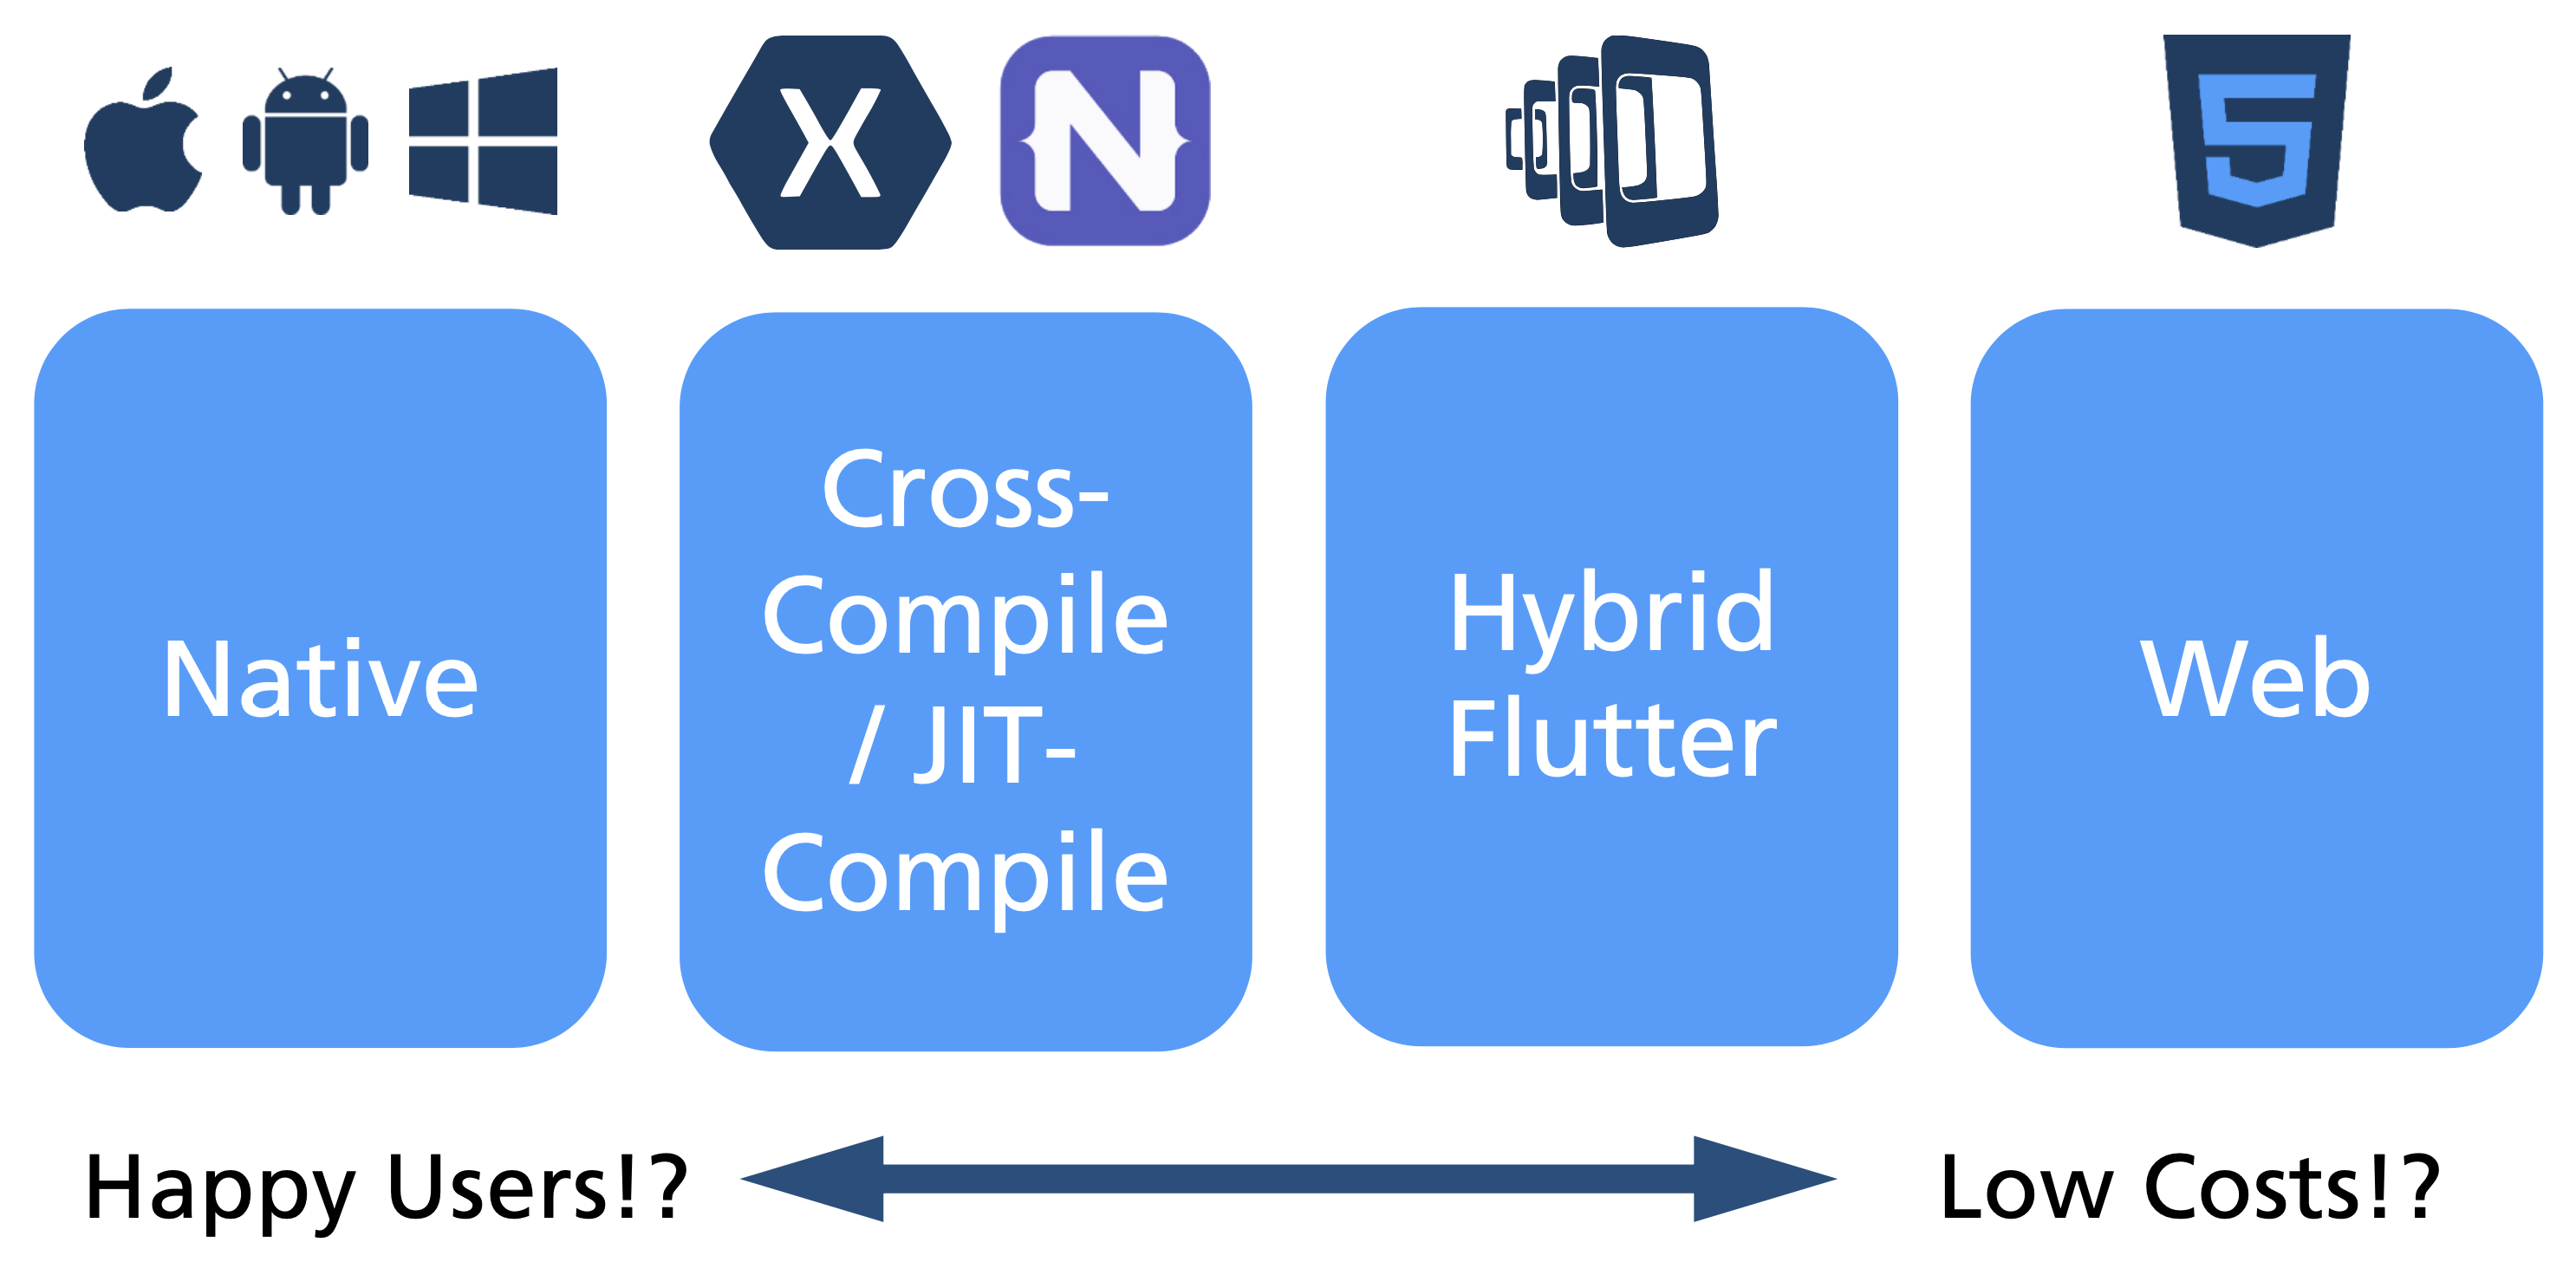
\includegraphics[width=0.7\textwidth]{img/techintro/spannungsfeld_apps.png}
			\caption{Das Spannungsfeld mobiler Entwicklung}
			\label{fig:techintro_spannungsfeld_apps}
		\end{figure}
	
		\begin{description}
			\item[Web-App] JS, HTML, CSS mit Responsive Design, im Browser ausgeführt
			\item[Hybrid] Web-App in nativem Wrapper verpackt, mit Connector-Plugins, kann als native App installiert werden (Cordova, Flutter etc.)
			\item[Cross-Compiled] In Sprache X geschriebene App, wird nach Java/Object-C oder binäres Format kompiliert und somit "native" (Xamarin, Ruby etc.)
			\item[JIT-compiled / VM] Javascript-App, läuft auf JS-Engine des Zielsystems und wird dort "just in time" kompiliert.
			Natives GUI und Konnektoren, um mit nativer Platform zu interagieren (NativeScript)
			\item[Native App] Spezifisch pro OS programmiert, nutzt volles Featureset der Plattform, auch neuste Features
		\end{description}
	
		\begin{figure}[htb!]
			\centering
			\includegraphics[width=.55\textwidth]{img/techintro/entwicklungsansätze.png}
			\caption{Übersicht mobiler Entwicklungsansätze}
			\label{fig:techintro_entwicklungsansätze}
		\end{figure}
	
		\newpage
	
		Welches ist jedoch der beste Ansatz für eine App?
		Immer abhängig von Anforderungen und Möglichkeiten.
		Mögliche Szenarien:
		
		\begin{itemize}
			\item Info-App ohne viel Interaktion $\rightarrow$ \textbf{Web-App}
			\item 100\% natives Look n Feel $\rightarrow$ \textbf{Nativ}
			\item Viele Plattformen nativ unterstützen, preiswert, .NET oder Angular Knowhow vorhande $\rightarrow$ \textbf{Cross-/JIT-Compile (Xamarin, NativeScript)}
			\item Gemeinsame Codebase, Crossplattform, eigene Widgets, Hot-Reload, kleine App / Prototyp $\rightarrow$ \textbf{Flutter}
			\item HW-Features benötigt auf verschiedenen Plattformen (NFC, Kamera, BT, Storage...) $\rightarrow$ \textbf{Hybrid / Nativ}
		\end{itemize}
	
		\subsection{Android Grundlagen}
		
		\begin{itemize}
			\item Android-Applikationen bestehen aus vier Komponenten:
			\begin{description}
				\item[Activity] UI-Komponente, entspricht typischerweise einem Bildschirm
				\item[Service] Komponente ohne UI, Dienst läuft typischerweise im Hintergrund
				\item[Broadcast Receiver] "Event-Handler", reagiert auf Broadcastsnachrichten (Intents)
				\item[Content Provider] Komponente, ermöglicht Datenaustausch zwischen versch. Applikationen
			\end{description}
			\item \textbf{Android Runtime (ART)} verwaltet die einzelnen Komponenten einer Applikation
			\begin{itemize}
				\item Mit Intent-Mechanismus kann eine Komponente eine andere Komponente aufrufen
				\item Komponenten müssen beim System registriert sein (teilweise Rechte = Privileges)
				\item System verwaltet Lebenszyklus von Komponenten (Gestartet, Pausiert, Aktiv, Gestoppt etc.)
			\end{itemize}
			\item Android empfiehlt für Hintergrundaufgaben nicht mehr Services, sondern \texttt{android.app.job.JobScheduler}\\
			Neu ist JobScheduler auch in WorkManager von Android Jetpack integriert
		\end{itemize}
	
			\subsubsection{Android Manifest}
			
			\begin{itemize}
				\item Beschreibt statische Eigenschaften einer Applikation
				\begin{itemize}
					\item Basis Java-Package-Name
					\item Benötigte Rechte (Internet, Kontakte etc.)
					\item Deklaration von Komponenten
					\begin{itemize}
						\item Activities, Services, Content Providers, Broadcast Receivers
						\item Name (+ Basis-Package = Java-Klasse)
						\item Anforderungen für Aufruf (Intent-Filter) für \textbf{A, S, BR}
						\item Format der gelieferten Daten für \textbf{CP}
					\end{itemize}
				\end{itemize}
				\item Diese Infos werden bei der App-Installation im System registriert
				\item Zusatzinfos (Version, ID etc.) befinden sich im Build-Skript (da diese build-abhängig sein können)
			\end{itemize}
		
			\subsubsection{Android Projekt-Struktur}
			
			\begin{itemize}
				\item Manifest
				\item Java-Code: Activities (App-Logik, Tests usw.)
				\item Ressourcen (\texttt{res})
				\begin{itemize}
					\item Bilder (\texttt{drawable})
					\item Layouts (\texttt{layout})
					\item Menus (\texttt{menu})
					\item Werte (\texttt{value})
				\end{itemize}
				\item Gradle Skripts (Angaben zum Build)
			\end{itemize}
		
		\newpage
		
		\subsection{Android Jetpack \& App-Architektur}
		
		Zwei massive Neuerungen in letzter Zeit:\\
		Seit 2019: Kotlin wird primäre Android-Sprache\\
		Seit 2018: Android Jetpack wird ins Leben gerufen
		
			\subsubsection{Android Jetpack}
			
			\begin{itemize}
				\item Sammlung von SW-Komponenten, die bei der Entwicklung von state-of-the-art Android-Applikationen unterstützen soll
				\item Jetpack-Komponenten im \texttt{androidx.}-Namespace, wurden teils aus Standard-API hierhin verschoben
				\item Alle Komponenten sind rückwärtskompatibel, können unabhängig von Android-Release-Zyklus aktualisiert und verwendet werden
				\item Jetpack wird von Google entwickelt und dokumentiert
			\end{itemize}
			\vspace{1em}
			Jetpack wird unterteilt in 4 Bereiche:
			\vspace{1em}
			\begin{itemize}
				\item Architecture
				\begin{itemize}
					\item Data Binding, Lifecycles, LiveData etc.
				\end{itemize}
				\item UI
				\begin{itemize}
					\item Animation/Transitions, Auto, TV, Wear, Emoji, Fragment etc.
				\end{itemize}
				\item Behavior
				\begin{itemize}
					\item Download Manager, Media \& Playback, Permissions, Notifications etc.
				\end{itemize}
				\item Foundation
				\begin{itemize}
					\item AppCompat, Android KTX, Multidex, Test
				\end{itemize}
			\end{itemize}
			
		\begin{figure}[htb!]
			\centering
			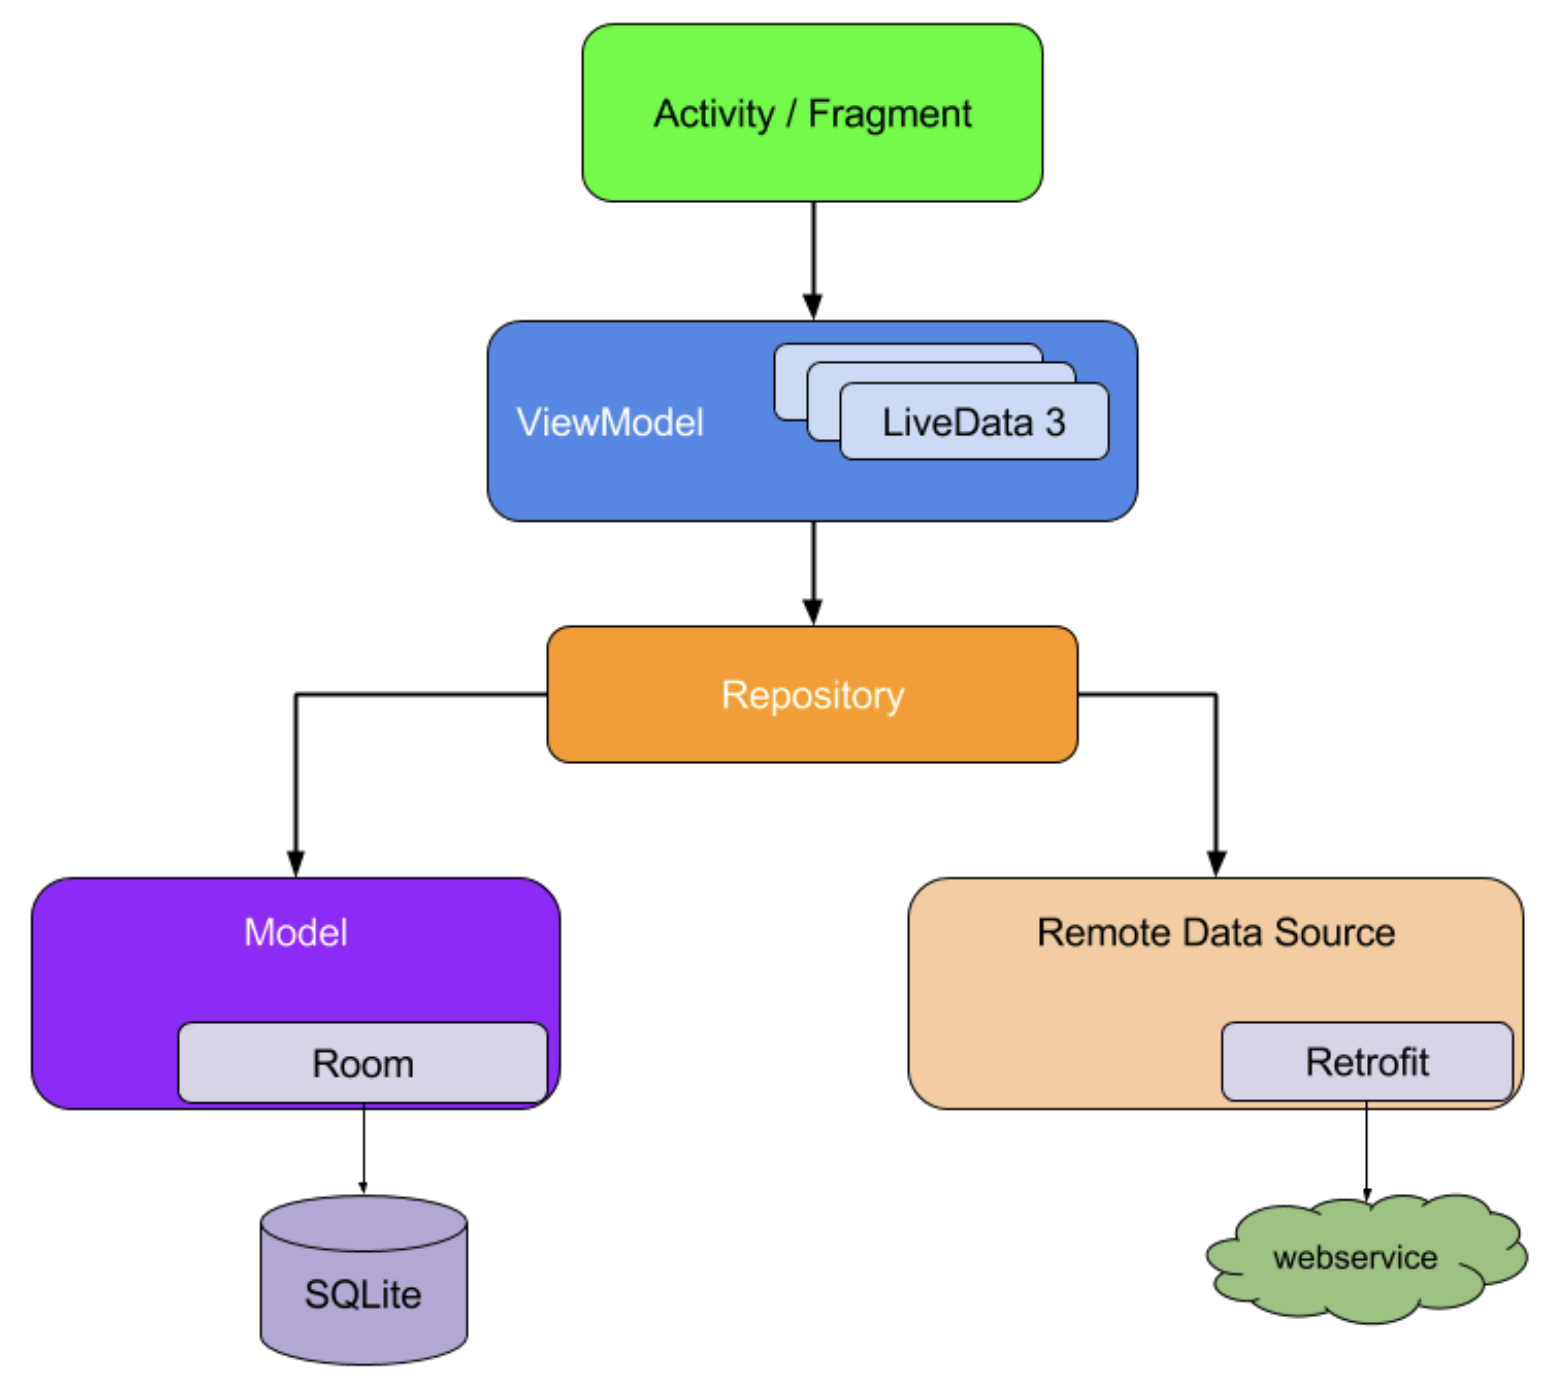
\includegraphics[width=0.5\textwidth]{img/techintro/apparch.png}
			\caption{Empfohlene App-Architektur}
			\label{fig:techintro_apparch}
		\end{figure}
		
		\newpage
		
			\subsubsection{Android Architecture Components (AAC)}
			
			\begin{itemize}
				\item Android Architecture Components enthalten eine Reihe von Lifecycle-bewussten Komponenten
				\item Komponenten helfen bei der Lösung von Problemen mit Konfigurationswechsel, Persistenz, Memory-Leaks und asynchronem Datenupdate auf dem UI
				\item AAC definieren seit 2017 eine standardisierte Vorgehensweise und stellen die offiziell empfohlene Lösung von Google dar
			\end{itemize}
		
			\begin{figure}[htb!]
				\centering
				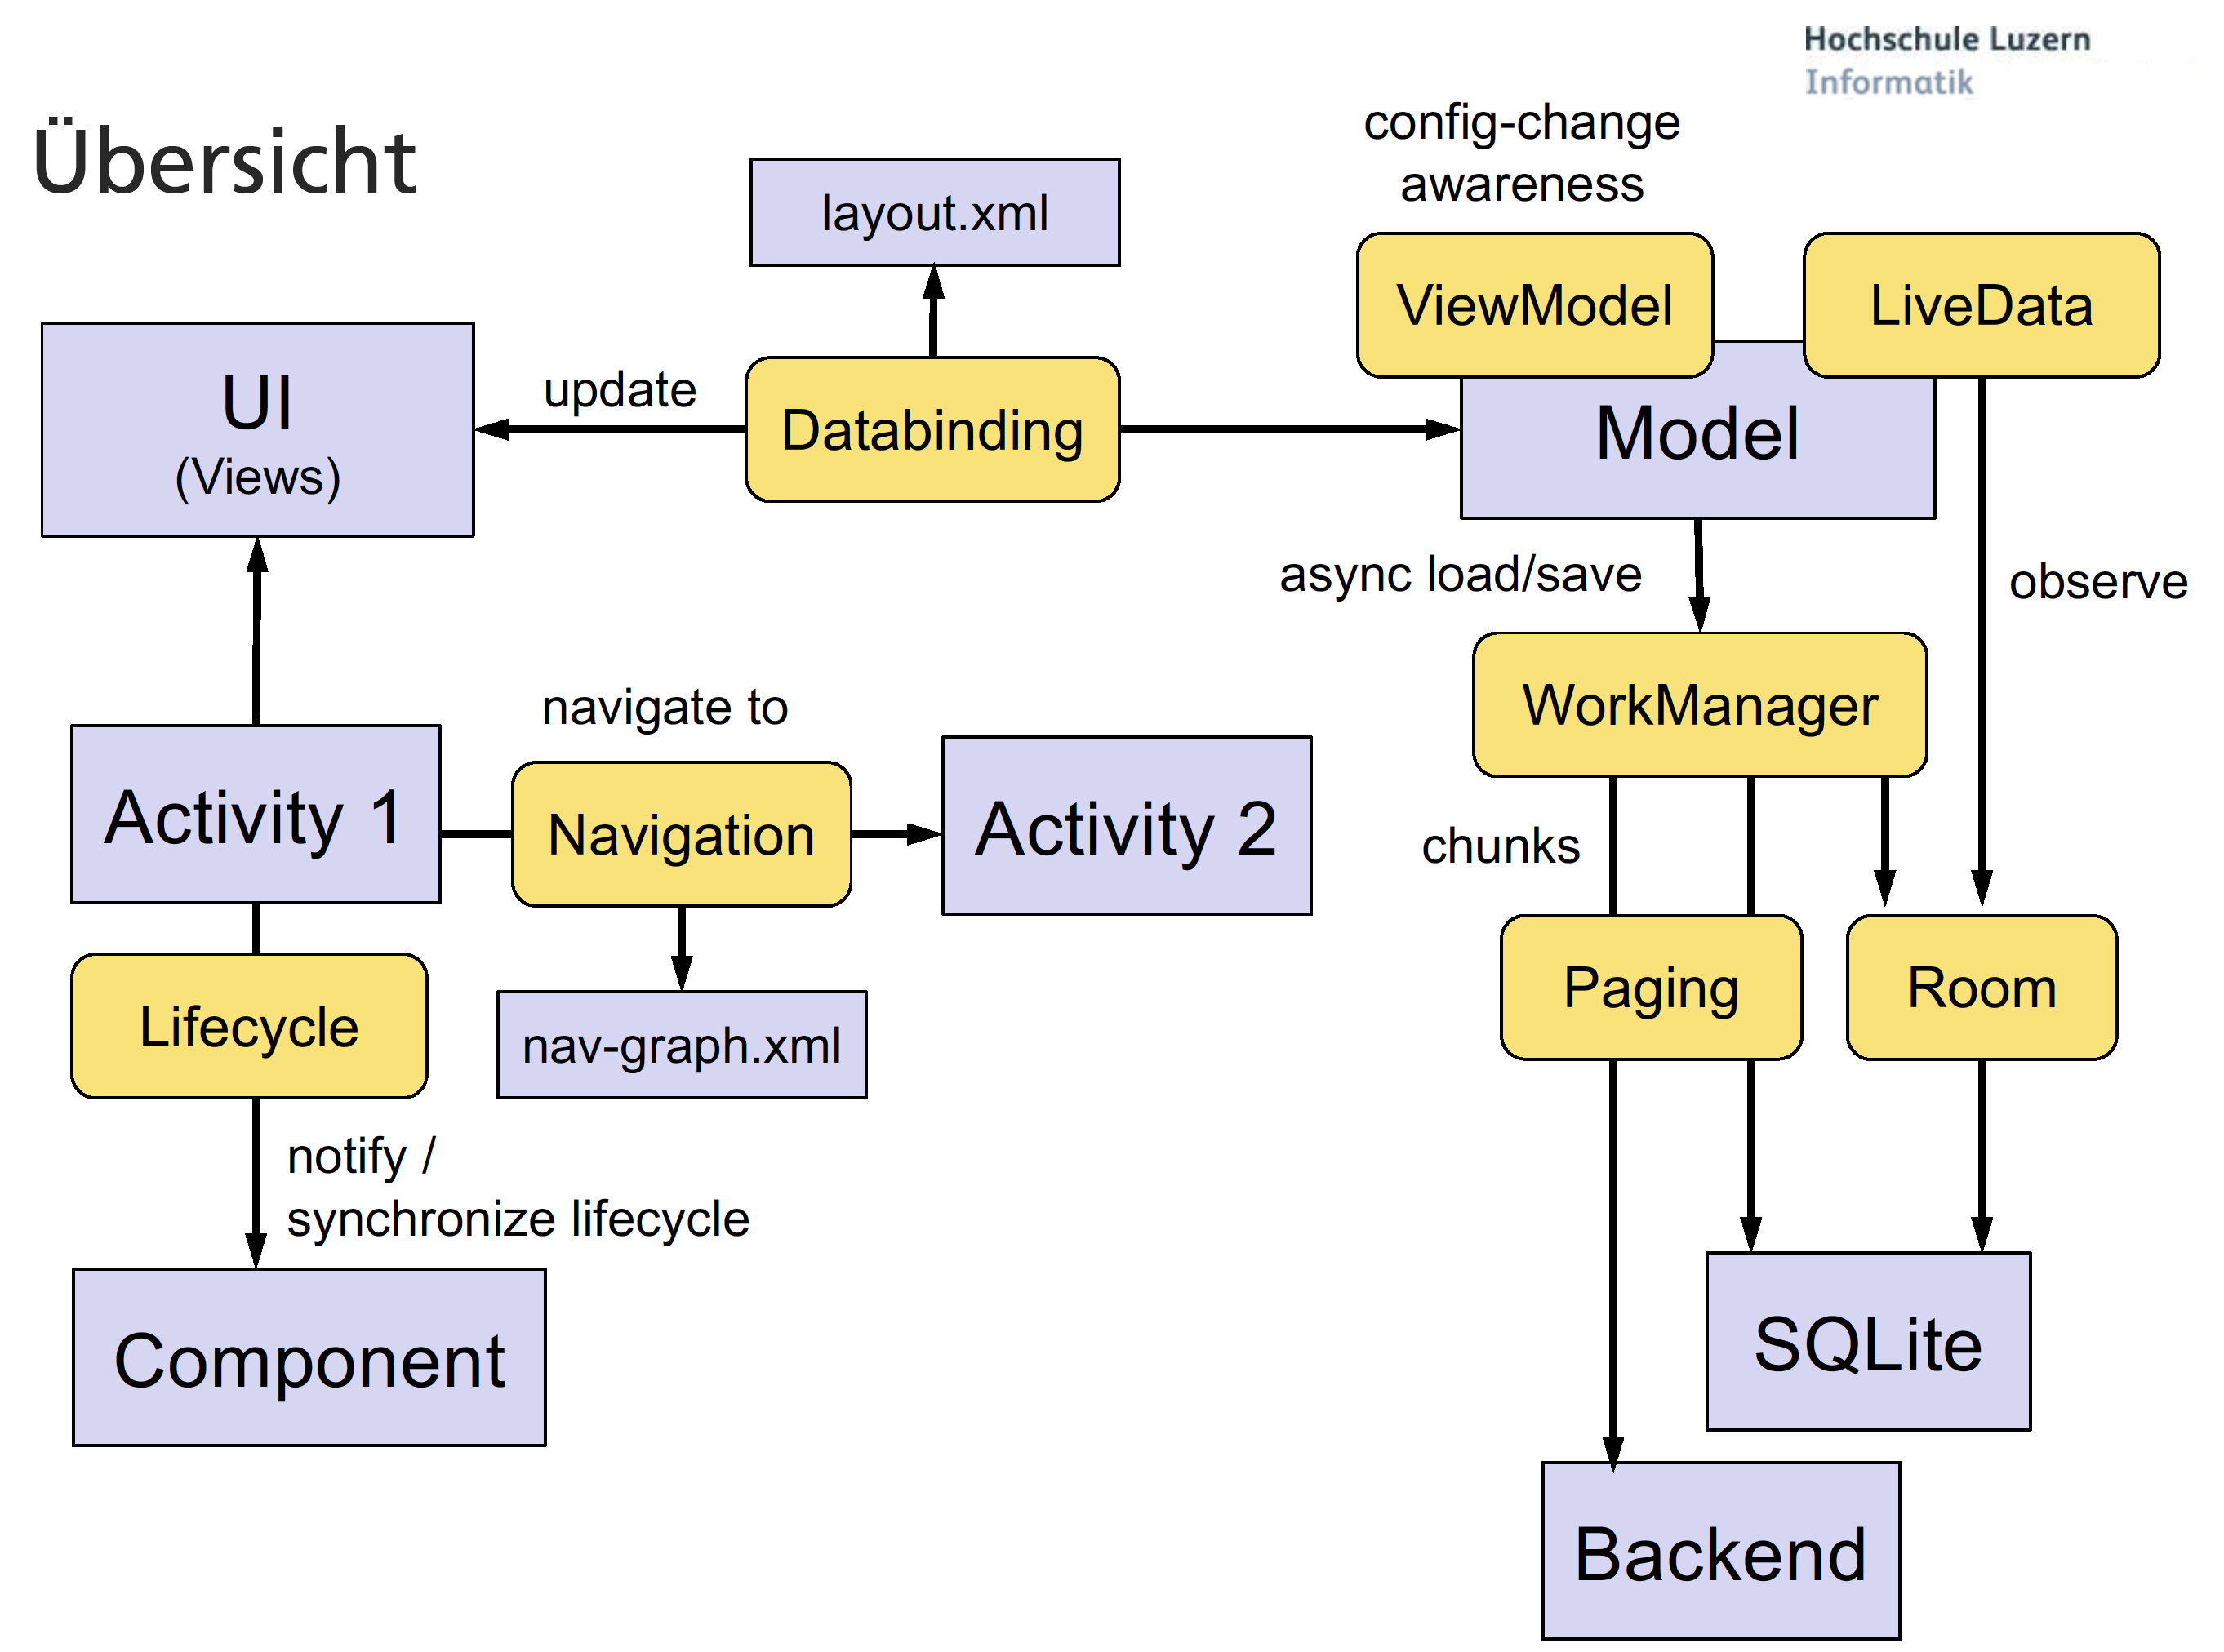
\includegraphics[width=0.7\textwidth]{img/techintro/overview_aac.png}
				\caption{Übersicht der Android Architecture Components}
				\label{fig:techintro_overview_aac}
			\end{figure}
		
				\paragraph{Data Binding}
				
				\begin{itemize}
					\item Separiert das UI von den Daten
					\item Synchronisiert UI mit Daten (1-way oder 2-way Binding)
					\item Verwendet "Binding Expressions" mit @{...} Syntax im Layout-File, um View-Attribute zu initialisieren
				\end{itemize}
			
				\paragraph{Lifecycle}
				
				\begin{itemize}
					\item Kann Code aus den Lifecycle-Hooks von Activities entfernen und direkt auf der beobachtenden Komponente implementieren.
					\item \texttt{Lifecycle} ist ein Objekt, welches den Lebenszyklus einer Komponente abbildet (Activity, Fragment etc.)
					\item Andere Komponenten können das Lifecycle-Objekt beobachten und auf Lifecycle-Events reagieren
				\end{itemize}
			
				\paragraph{LiveData}
				
				\begin{itemize}
					\item Updates können im Hintergrund erfolgen, werden aber nur ausgeführt, wenn der Observer der LiveData in einem aktiven Zustand ist (\texttt{STARTED, RESUMED})
					\item \texttt{LiveData} ist eine lifecycle-aware Observable-Klasse
					\item Kann als Source für Data Binding verwendet werden, um Aktualisierungen des UI während der Laufzeit zu forcieren
				\end{itemize}
			
				\paragraph{Navigation}
				
				\begin{itemize}
					\item Android gibt neu Navigationsprinzipien vor, hierbei hilft die \texttt{Navigation}-Komponente bei der Implimentierung dieser Prinzipien
					\item \texttt{Navigation} basiert Navigation-Graph (Resources) mit Destinations (Knoten) und Actions (Kanten)
						\textit{(Navigation-Graph wird von Hand oder mit Navigation-Editor in Android Studio erstellt)}
					\item Navigation benötigt \texttt{NavHostFragment} im Layout (um die Zielfragmente einzublenden);
					Aus dem Code heraus wird mit einer \texttt{NavController}-Instanz navigiert
				\end{itemize}
			
				\paragraph{Paging}
				
				\begin{itemize}
					\item Es müssen nicht alle Daten auf einmal geladen werden: schneller und weniger Load
					\item Unterstützt asynchrones Laden von Daten
					\item \texttt{PagedList} und \texttt{PagedListAdapter}, um bei Bedarf weitere Daten in einer \texttt{RecyclerView} zu laden
				\end{itemize}
			
				\paragraph{Room}
				
				\begin{itemize}
					\item Bessere Abstraktion, Speichern/Laden von Modellobjekten, kein handgestricktes SQL-Mapping
					\item Room ist ein ORM (Object-Relational Mapper) für SQLite
					\item Arbeit mit Entities (Modell-Objekten) und DAO-Pattern anstatt SQL
				\end{itemize}
			
				\paragraph{ViewModel}
				
				\begin{itemize}
					\item Weniger Aufwand für Behandlung von Konfigurationsänderungen (keine Serialisierung nötig)
					\item Kapselt UI-Daten so, dass sie bei Konfigurationsänderung einer Activity in-memory erhalten bleiben
					\item Aber: Für den Fall eines App-Kills durch das OS müssen Daten immer noch persistiert werden!
				\end{itemize}
			
				\paragraph{WorkManager}
				
				\begin{itemize}
					\item Kein Kopfzerbrechen über Regeln für Hintergrundtasks, Synchronisation von UI via LiveData
					\item \texttt{WorkManager} führt asynchrone \texttt{WorkRequests} sofort oder zu geeignetem Zeitpunkt aus
					\item Respektiert Doze-Mode, versucht Ressourcen zu sparen und Load zu minimieren.
						Je nach Zustand von App/System werden Tasks unterschiedlich scheduled.
					\item Pro WorkRequest wird ein LiveData-Objekt erzeugt, Zustand und Daten sind darüber beobachtbar
				\end{itemize}\textbf{}
			
				\paragraph{App-Architektur: Tipps \& Empfehlungen}
				
				\begin{itemize}
					\item Standards / Patterns soweit möglich benutzen
					\item Aber: Kein Over-Engineering!
					\item Alle AAC können einzeln oder zusammen verwendet werden
					\item Herausfinden, was im Projekt am besten funktioniert bzw. am meisten Sinn macht
					\item Vorsicht bei Background-Tasks
					\begin{itemize}
						\item System zunehmend restriktiver, grosse Änderungen mit API 26
						\item "Background = Service" gilt nicht mehr
						\item WorkManager meist die bessere Alternative, Service für Logikexport 
					\end{itemize}
				\end{itemize}
				
	\newpage	
		
	\section{SA - Kotlin \& Android}
	\label{section:kotlin} 
	
		\subsection{Sprachübersicht}
		
			\begin{itemize}
				\item Variablen zwingend mit \texttt{var} (veränderbar) oder \texttt{val} (unveränderbar) kennzeichnen
				\item Primitive Datentypen gibt es nicht, dafür Klassen für diese (Int, Double etc.)
				\item Kontrollstruktur-Ausdrücke haben immer einen Wert
				\item Keine checked Exceptions
				\item Strichpunkt am Ende einer Zeile ist optional
				\item Typinferenzen, weniger explizite Typangaben als bei Java
				\item Nullable-Typen können gegen NullPointerExceptions vorbeugen
				\item Mit Extensions Klassen ohne Vererbung erweitern
				\item Data Classes für kompakte Klassendeklaration inkl. automatisch implementierten equal / toString / hashCode Methoden
			\end{itemize}
	
		\subsection{Spracheigenschaften (eine Auswahl)}
		
			\paragraph{Variablen-Deklaration: var, val \& Typinferenz}
			\begin{itemize}
				\item \texttt{var} (veränderbar) und \texttt{val} (unveränderbar)
				\item Typangaben können grundsätzlich weggelassen werden \\
					(Compiler erkennt Datentyp automatisch und weist diesen korrekt zu)
				\item Java kennt für lokale Variablen seit 2018 ähnliche var-Syntax mit Typinferenz für lokale Variablen
				\item Bei Kotlin: Typangabe nach dem Namen\\
					Bei Java: Typangabe vor dem Namen
			\end{itemize}
		
			\paragraph{Nullable-Typen, Safe-Calls \& Elvis-Operator}
			\begin{itemize}
				\item In Kotlin können jegliche Typen nie den Wert null annehmen\\ 
					(ausser sie werden explizit als nullable deklariert)
				\item Variable, die Wert null zulassen soll, so deklarieren mit \texttt{[type]?}
				\item Nullable-Variablen können nicht direkt abgerufen werden (könnte ja null sein)
				\begin{itemize}
					\item Variable entweder erst auf null überprüfen
					\item Safe-Call Operator \texttt{?.} nutzen (druckt Wert der Variable oder null)
					\item Not-Null-Assertion-Operator \texttt{!!} (wirf NullPointerException, falls Wert null ist)
				\end{itemize}
				\item Spezialfall: falls nicht-null, nimm den Wert und sonst X
				\begin{itemize}
					\item Elvis-Operator \texttt{?:} (folgend auf diesen kann ein Wert angegeben werden)
					\item Zusammen mit Safe-Call-Operator nützlich, da so ein Alternativwert angegeben werden kann, falls eine Variable doch null sein sollte
				\end{itemize}
			\end{itemize}
		
			\paragraph{Funktionen: Benannte Parameter \& Default-Werte}
			\begin{itemize}
				\item Schlüsselwort \texttt{fun} zur Deklaration von Funktionen
				\item Benannte Parameter und Default-Werte für Parameter
				\begin{itemize}
					\item Benannte Parameter für bessere Lesbarkeit
					\item Default-Werte für übersichtliche Aufrufe
					\item Bei Aufruf einer Funktion mit bennanten Parametern können diese beliebig angeordnet werden, 
					jedoch darf beim Aufruf nicht zwischen unbenannt und benannt gemischt werden, da sonst die Position der Parameter nicht mehr stimmen könnte
				\end{itemize}
				\item Default-Werte helfen bei der Code-Einsparung (bei Java brucht es bei x Parametern x Methoden)
				\item Weitere spannende Möglichkeiten von Funktionen:\\
					\texttt{tailrec} für endrekursive Funktionen, Funktionen mit nur einem Ausdruck, Funktionen mit expliziten Rückgabetypen, Modifier \texttt{infix} für infix-Aufrufe (infix-Notation und ohne Klammern)
			\end{itemize}
		
			\paragraph{Extension: Erweiterung ohne Vererbung}
			\begin{itemize}
				\item Extensions, um bestehende oder auch fremde Klassen um Funktionen zu erweitern\\
					z.Bsp. kann Klasse \texttt{Int} um Funktion \texttt{myPrettyPrint()} erweitert werden
			\end{itemize}
	
		\newpage	
	
		\subsection{Kotlin \& Android}
		
		\begin{itemize}
			\item Kotlin offizielle Androidsprache, da kompakt, ausdrucksstark, Typ- und Null-sicher
			\item Parallele Verwendung von Java und Kotlin möglich für Android-Entwicklung
			\item Aus Kotlin-Klasse kann auf Java-Klasse zugegriffen werden (und umgekehrt)
			\item Sicherer als Java dank non-nullable Typen und kompakteren Konstrukten \\
				40\% weniger Zeilen Code als bei Java
			\item Android findViewById() entfällt bei Kotlin, da direkt Extension-Properties für alle id's in Ressourcen-Dateien angelegt werden, so kann direkt auf jede id zugegriffen werden
		\end{itemize}
		
	\section{SA - Data Binding \& ViewModel}
	\label{section:databinding}
	
		\subsection{Kontext}
		
		\begin{itemize}
			\item Eine Activity ist ein Bildschirm, zu jeder Activity gehört ein UI-Layout in einem XML, welches darzustellende Views definiert
			\item UI-Initialisierung in der \texttt{onCreate()} einer Activity
			\item Code mit Zuständigkeit für Daten, UI und Eventhandling wird vermischt
			\item Data Binding soll Daten und UI strikt trennen
			\item ViewModel soll Behandlung von Konfigurationsänderungen von der Activity separieren
		\end{itemize}
	
		\subsection{Data Binding}
		
		\begin{itemize}
			\item Anbindung eines Datenmodells an UI-Komponente
			\item Modell für UI-Daten erzeugen und mit UI verbinden
			\item \textit{One-Way-Binding}: Wird Datenmodell modifiziert, aktualisiert UI automatisch mit neuen Daten
			\item \textit{Two-Way-Binding}: Auf UI eingegebene Daten werden auch mit dem Modell synchronisiert
			\item Eliminiert viel Listener- und Update-Code in den Activity-Klassen
			\item Test- und Wartbarkeit wird erhöht, im Best Case nur noch Modell-Logik testen
			
			\item Data Binding über spezielle Layout-Files definieren
			\begin{itemize}
				\item \texttt{<layout>} mit zwei Unterelementen
				\begin{itemize}
					\item \texttt{<data>}: deklariert Namen und Typen der verwendeten Datenquellen
					\item \texttt{View}: entspricht Root-Komponente eines normalen Layout-Files
				\end{itemize}
				\item Für beliebige Attribute von View-Elementen Binding-Expressions definierbar\\
					(werden zum Zeitpunkt der Instanzierung ausgewerten und deren Resultat als Wert des Attributs gesetzt)
				\item Binding-Expressions innerhalb des Markers \texttt{@{...}} definiert, können auf Variablen/Modellobjekte referenzieren, welche im <data> Element des Layouts definiert worden sind
				\item Binding-Expressions können auch einen Default-Wert enthalten (falls sie Null sind)
			\end{itemize}
			\item Model-Klasse implementiert definierte Properties, am besten als public-Felder
			\item Klassen werden automatisch generiert, welche die Binding-Logik für jedes Layout implementieren (mit Suffix \textit{Binding} nach dem Activity-Namen)
			\item Initialisierung des UI mit \texttt{DataBindingUtil.setContentView()} in \texttt{onCreate()}\\
				Die Model-Klasse wird ebenfalls hier geladen, mit Werten belegt und gebunden
			\item Observables für Aktualisierungen in der Model-Klasse definieren
		\end{itemize}
	
		\subsection{ViewModel}
		
		\begin{itemize}
			\item ViewModel, um den mit UI verbundenen Zustand in-memory zu speichern
			\item Mit Data Binding kombinierbar, da Data Binding nach erneuter Initialisierung der Activity sonst den Wert null oder Default-Werte wieder annimmt
			\item ViewModel-Klasse erstellen, welche von ViewModel ableitet / erbt
			\item Hier Observables definieren, mit den zu überwachenden UI-Elementen
			\item ViewModel-Klasse muss mit der Activity verbunden werden, mit welches es seine Daten synchronisiert (\texttt{ViewModelProviders})
			\item ViewModel muss einen Default Konstruktor haben, welcher eine Application als Argument nimmt, für den Fall von AndroidViewModel
			\item Bei Verbindung mit Backend / DB überprüfen, ob diese schon einmal geladen worden, da ansonsten das ViewModel zurückgesetzt wird wenn keine Verbindung zum Backend besteht, was unerwünscht ist
		\end{itemize}
		
	
	\section{SA - Fastlane}
	\label{section:fastlane}
	
		\subsection{Übersicht}
		
		\begin{itemize}
			\item Fastlane als Tool zur Automatisierung von Apps
			\item Gefördert von Google und optmiert für macOS, da Basisfunktionalitäten auch für Automatisierung von iOS-Apps benötigt wird (nur auf macOS möglich)
			\item Im Kern eine Sammlung nützlicher Ruby-Skripts, Funktionalität kann um Plugins oder eigene Skripte einfach erweitert werden
			\item Standardfunktionen beinhalten Kompilation und Signierung von Apps, Ausführen von Tests, Anpassen von Metainformationen, Erstellen von App-Screenshots, Veröffentlichungen in App-Stores, Versenden von Statusmeldungen via Slack, Twitter etc.
		\end{itemize}
	
		\subsection{Installation}
		
		\begin{itemize}
			\item Fastlane ist nur eine Wrapper um bestehende Werkzeuge, unterteilt in \textbf{Fastlane Actions}
			\item Nebst einer Ruby-Installation werden Basis-Entwicklerwerkzeuge vorausgesetzt \\
				(Android SDK für Android, Xcode für iOS etc.)
			\item Zur Versionierung der verwendeten Ruby-Pakete wird \texttt{Bundler} benutzt \\
				Bundler speichert alle pro Projekt verwendeten Pakete mit Versionsnummern, ermöglicht somit Wiederherstellung aller Abhängigkeiten			
		\end{itemize}
	
		\subsection{Grundwissen zu Fastlane}
		
		\begin{itemize}
			\item Fastlane unterstützt neben Android und iOS auch andere Tools wie Xamarin dank Plugins
			\item Die minimale Struktur des Grundgerüsts von Fastlane beinhaltet folgende Dateien \\
				(Diese sollten in einem Versionskontrollsystem verwaltet werden, damit spätere Reproduzierbarkeit mit den exakten Abhängigkeiten gewährleistet wird):			
			\begin{description}
				\item[Gemfile] Liste aller verwendeten Ruby-Pakete
				\item[Gemfile.lock] Speichert Versionsnummer aller verwendeten Ruby-Pakete
				\item[Appfile] Konfigurationsparameter der zu automatisierenden App
				\item[Fastfile] Enthält Anweisungen und Aktionen für Fastlane, Haupttätigkeit bei der Automatisierung ist die Anpassung dieser Datei
			\end{description}
			\item Bundler analysiert Gemfile und Gemfile.lock zur Wiederherstellung der Ruby-Pakete
			\item Fastlane wird ebenfalls verwaltet, weshalb immer die lokale Fastlane-Installation genutzt werden sollte: 
				\texttt{bundle exec fastlane [parameters]}
			\item Strukturierung des Fastfile:
			\begin{itemize}
				\item \texttt{Platforms}: Oberste Schicht, beschreibt Plattform (Android, iOS)
				\item \texttt{Lanes}: genauere Unterteilung, evtl. nach Funktion, Tätigkeit, fasst Actions zusammen
				\item \texttt{Actions}: wiederverwendbare Automatisierungsschritte
			\end{itemize}
		\end{itemize}
	
		\subsection{Fortgeschrittene Themen}
		
		\paragraph{Actions \& Plugins}
		\begin{itemize}
			\item Actions können auch direkt über das CLI ausgeführt werden\\
				\texttt{bundle exec fastlane run [action-name] [parameters]}
			\item 221 Standard-Aktionen in Fastlane, diese können um Plugins erweitert werden, welche über das CLI oder die Webseite gesucht werden können \\
				Plugins suchen: \texttt{bundle exec fastlane search\_plugins [search-term]} \\
				Plugins installieren: \texttt{bundle exec fastlane add\_plugin [plugin-name]}
			\item Hilfe über eine Action (Beschreibung, Umgebungsvariablen etc.) können abgefragt werden: \\
				\texttt{bundle exec fastlane action [action-name]}
			\item Neue Actions können ebenfalls erstellt werden: \\
				\texttt{bundle exec fastlane new\_action}
			\item Neue Actions, welche veröffentlich werden sollen, am besten in eigenem Plugin erstellen. 
				Dieses soll in einem eigenen Verzeichnis erstellt werden, da es unabhängig vom Projekt sein soll: \\
				\texttt{fastlane new\_plugin [plugin-name]}
			\item Ist das Plugin publiziert, kann es dem Projekt hinzugefügt werden:
				\texttt{bundle exec fastlane add\_plugin [plugin-name]}
			\item Ein Plugin kann mit demselben Befehl auch vor der Publizierung eingebunden werden.
				Nach Eingabe des Befehls fragt Fastlane dann nach dem Pfad des Plugins.
		\end{itemize}
	
		\paragraph{Parameterisierung von Actions}
		\begin{itemize}
			\item Actions können Parameter direkt bei Eingabe im CLI entgegennehmen
			\item Actions besitzen Umgebungsvariablen, diese können abgefragt werden: \\
				\texttt{bundle exec fastlane action [action-name]}
			\item Wird der Umgebungsvariable ein Wert zugeteilt, nutzt Fastlane beim Aufruf der Action ohne mitgegebene Parameter diesen auf
			\item Fastlane kennt auch \texttt{.env} Dateien, in welcher Umgebungsvariablen eingetragen werden können (nützlich für Publizierung oder Zusammenarbeit) $\rightarrow$ werden nur bei \textbf{Ausführung einer Lane} genutzt!
			\item Für bspw. Test-Automatisierung können verschiedene .env Dateien erstellt und genutzt werden \\
				Bsp. \texttt{.env.test} $\rightarrow$ \texttt{bundle exec fastlane [lane] --env test}
		\end{itemize}
	
	\section{SA - Unreal Engine}
	\label{section:unrealengine}
	
	
	\section{SA - Xamarin.Forms}
	\label{section:xamarinforms}
	
		\subsection{Xamarin \& Entstehung}
	
		\begin{itemize}
			\item Xamarin ist ein Open-Source-Framework, ermöglicht Entwicklen von Apps für Android und iOS mittels C\# und .NET
			\item Bisher musste das UI native pro Plattform erstellt werden, Xamarin-Projekte konnten sich nur die "Businesslogik" teilen
			\item Xamarin.Forms soll ermöglichen, das UI für beide Plattformen zu vereinen, dass ebenfalls der Code für das UI geteilt wird
			\item Xamarin Apps werden mithilfe des Mono Execution Frameworks ausgeführt (auf Android läuft dazu eine zusätzliche VM auf welche ART zugreift, während auf iOS Bindings des Mono EE auf die Native SDK existieren)
		\end{itemize}
	
		\subsection{Xamarin.Forms}
		
		\paragraph{Essentials \& Head Projects}
		\begin{itemize}
			\item Xamarin.Essentials bieten viele Grundfunktionalitäten, welche plattformspezifische Funktionalitäten in einer Library vereint (bspw. Zugriff auf Accelerometer, KeyStore/KeyChains usw.)
			\item Typisch gibt es 3 Projekte bei einem Xamarin-Projekt: das normale und 2 mit einem Suffix pro Plattform (diese werden Head Projects genannt)
			\item In den Head Projects sind MainActivity (Android) und AppDelegate sowie Main.cs (iOS), über welche eine Referenz des Hauptprojekts weitergegeben wird und die App geladen wird.
			Hier befindet sich ebenfalls plattformspezifischer Code, welcher nicht geteilt genutzt werden kann.
		\end{itemize}
	
		\vspace{1em}
		
		\begin{itemize}
			\item XAML wurde hauptsächlich für das Designen von UIs entwickelt
			\item Jedes XAML besitzt ein Code-behind File, welches die Logik für das UI beinhaltet
			\item Typ bzw. Technologie am Anfang des XAML definieren (hier Xamarin)
			\item UI kann mittels Properties im XAML verändert werden oder auch über C\#-Code
			\item Event Handling: Bester Weg ist, im XAML Properties als x:[Type] zu deklarieren und über Code auf diese zuzugreifen (besser für Separation of Concerns)
			\item Plattformspezifische Werte können im code-behind oder XAML angegeben werden (falls eine Plattform gewisse UI-Elemente anders anzeigen sollte)
			\item Head Projects müssen angepasst werden, wenn gewisse Logik eine plattformspezifische Anpassung benötigt (Hintergrundwissen der Plattformen sollte dazu für beide Plattformen etwas vorhanden sein)
		\end{itemize}
	
	\section{SA - PWA: Progressive Web Apps}
	\label{section:pwa}
	
	
\end{document}
